\section{Data Model}
\subsection{Scenario}
The scenario object will contains collections of top level objects that can be included in scenarios, including rooms, characters, conversations, and items. It will also contain JSON that will keep track of the player's progress in a scenario, which will be combined with the  other scenarios loaded in the current play session. Refer to Appendix~\ref{app:DataModel} for a detailed diagram describing the entire data model of \ourgame{}'s scenarios. The following describes the attributes of objects involved in the data model.

\begin{description}
\item[name]{the name of the scenario}
\item[description]{a description of the scenario}
\item[rooms]{a collection of rooms included in the scenario}
\item[chracters]{a collection of characters included in the scenario}
\item[conversations]{a collection of conversations included in the scenario}
\item[items]{a collection of items included in the scenario}
\item[saveFileJson]{JSON data related to the current state of the scenario}
\end{description}

\begin{figure}[H]
\label{fig:conceptual_data_model}
\centering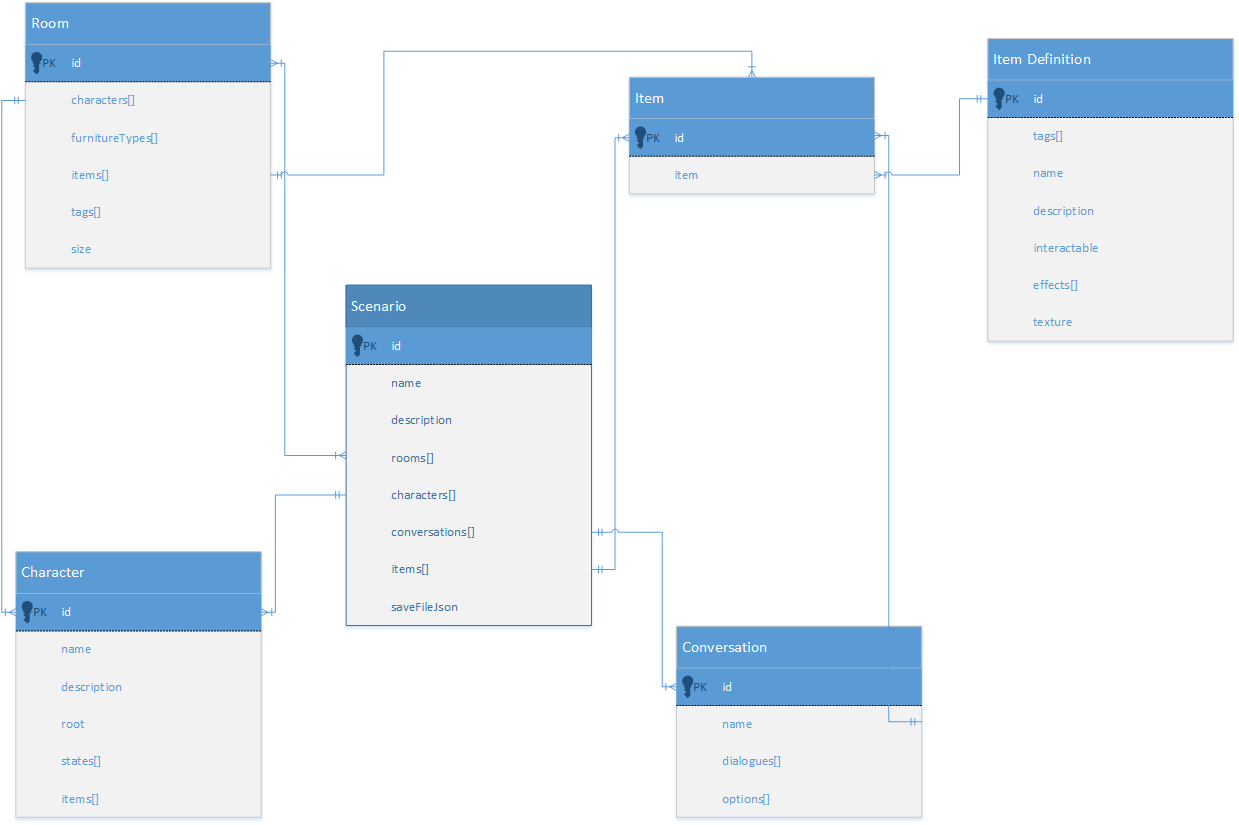
\includegraphics[width=.7\linewidth]{images/Conceptual_DataModel}
\caption{Conceptual Data Model of Scenarios}
\end{figure}

\subsection{Tag}
\begin{description}
\item[name]{the name of the tag}
\item[description]{a description of the tag}
\end{description}

\subsection{Character}
\begin{description}
\item[name]{the name of the character}
\item[description]{a description of the character}
\item[root]{the skeletal connection to the root component of the character (e.g. pelvis)}
\item[states]{a collection of states the character can be in during a scenario}
\item[items]{a collection of items a character possesses}
\end{description}

\subsubsection{Skeletal Connection}
\begin{description}
\item[component]{a character component}
\item[outComponents]{a collection of child Character Components of this object's own Character Component}
\end{description}

\subsubsection{Character Component}
\begin{description}
\item[name]{the name of the component}
\item[texture]{the URL of the image of the component}
\item[inJoint]{joint where the Character Component can be attached to}
\item[outJoints]{a collection of joints where child components can attach themselves to}
\item[tags]{a collection of tags that the component can be selected by}
\end{description}

\subsection{Conversation}
\begin{description}
\item[name]{the name of the conversation}
\item[dialogues]{a collection of dialogues spoken in the conversation by NPCs}
\item[options]{a collection of possible choices the player can choose at the end of a conversation}
\end{description}

\subsubsection{Dialogue}
\begin{description}
\item[speaker]{the character who will speak the dialogue}
\item[lines]{a collection of text to be spoken, separated by a \textbf{Next} button}
\item[triggerCalls]{a collection of calls to a trigger}
\item[conditionChecks]{a collection of conditions that can call a trigger if the condition is met}
\end{description}

\subsubsection{Trigger}
\begin{description}
\item[name]{the name of the trigger}
\item[description]{a description of the trigger}
\item[numArgs]{number of arguments the trigger is expecting}
\end{description}

\subsubsection{Trigger Call}
\begin{description}
\item[triggerId]{the id of the trigger to be called}
\item[arguments]{arguments to be sent to the trigger}
\end{description}

\subsubsection{Option}
\begin{description}
\item[text]{the option to be displayed to the player}
\item[link]{a reference to a conversation that will follow if the player chooses this option. If empty, the conversation ends and the Dialogue UI will close.}
\end{description}

\subsection{Item}
\begin{description}
\item[item]{a definition object containing properties of the item}
\end{description}

\subsubsection{Item Definition}
\begin{description}
\item[tags]{a collection of tags the item can be selected by}
\item[name]{the name of the item}
\item[description]{a description of the item}
\item[interactable]{a flag indicating whether the object can be picked up}
\item[effects]{a collection of effects the item can have on the scenario it belongs to}
\item[texture]{a URL to the image of the item}
\end{description}

\subsection{Room}
\begin{description}
\item[characters]{a collection of characters inside the room}
\item[furnitureTypes]{a collection of furniture inside the room}
\item[items]{a collection of items inside the room}
\item[tags]{a collection of tags describing the room type}
\item[size]{the dimensions of the room}
\end{description}

\subsubsection{Furniture Components}
\begin{description}
\item[name]{the name of the furniture component}
\item[meshUrl]{the path to the furniture component mesh}
\item[connections]{a collection of locations as to where the component should connect at}
\item[tags]{a collection of tags the furniture component can be selected by}
\item[types]{a collection of Furniture Types that can use the furniture component}
\end{description}

\subsubsection{Furniture Type}
\begin{description}
\item[tags]{a collection of tags describing the furniture}
\item[name]{then name of the furniture}
\end{description}

